%%%%%%%%%%%%%%%%%%%%%%%%%%%%%%%%%%%%%%%%%%%%%%%%
% COPYRIGHT: (C) 2012-2015 FAU FabLab and others
% CC-BY-SA 3.0
%%%%%%%%%%%%%%%%%%%%%%%%%%%%%%%%%%%%%%%%%%%%%%%%


\newcommand{\basedir}{fablab-document}
\documentclass{\basedir/fablab-document}

% \usepackage{fancybox} %ovale Boxen für Knöpfe - nicht mehr benötigt
\usepackage{amssymb} % Symbole für Knöpfe
\usepackage{subfigure,caption}

\usepackage{eurosym}
\usepackage{tabularx} % Tabellen mit bestimmtem Breitenverhältnis der Spalten
\usepackage{wrapfig} % Textumlauf um Bilder
\usepackage[ngerman]{cleveref} % einfachere Referenzierung: \cref{foo} erzeugt z.B. "Kapitel 7" oder "Abbildung 5" je nach Typ der Referenz
\renewcommand{\texteuro}{\euro}

\linespread{1.2}

\date{\today}
\author{Max, Philipp, Michael u.a.}
\fancyfoot[L]{kontakt@fablab.fau.de}
\title{Grundlagen-Einweisung Fräse}

\tikzstyle{knopf} = [anchor=base, draw=black, fill=gray!10, rectangle, rounded corners, inner sep=2pt, outer sep = 3pt]

\newcommand{\knopfStyled}[2]{
    \begin{tikzpicture}[baseline={(box.base)}]
    \node [#1] (box) { 
        \fontsize{9pt}{9pt}\selectfont \textbf{#2}\strut
    };
    \end{tikzpicture}
}

\newcommand{\knopf}[1]{\knopfStyled{knopf}{#1}}
\newcommand{\cncStart}{\knopf{Start}}

%\tikzstyle{todo} = [knopf, draw=white, fill=yellow]
%\newcommand{\todo}[1]{\knopfStyled{todo}{#1}}
\renewcommand{\todo}[1]{\colorbox{yellow}{{#1}}}

\usetikzlibrary{shadows}
\usetikzlibrary{decorations}
\begin{document}
\section{Regeln und Hinweise}\label{regeln}
\subsection{Was darf ich?}
Ohne eine unterschriebene Grund-Einweisung in diese Regeln darf die Fräse nicht benutzt werden, d.h. du darfst \emph{garnichts} an/in der Fräse und dem zugehörigen Steuerrechner tun.
\begin{itemize}
 \item Jede Einweisung verfällt nach einem Jahr, wenn sie nicht vorher schriftlich erneuert wurde. 
 \item Mit Grund-Einweisung darfst du den Fräs-Auftrag zwar selber vorbereiten (Werkstück einspannen), \textbf{die Steuerung aber nicht selbstständig bedienen, also die Maschine nicht \enquote{fahren lassen}}.
 \item Alles andere darfst du zuerst nur unter ständiger Aufsicht durch einen Experten. Mit jedem Fräsen lernst du dazu und darfst dann immer mehr selbstständig tun, sobald es dir \textbf{schriftlich} erlaubt wird:
 %\item Die Bedienung der Steuersoftware (Antasten, Starten, Fortsetzen nach Pause, ...) darf nur durch den Experten bzw. unter ständiger Aufsicht durch den Experten erfolgen.
\end{itemize}
\colorlet{blockhintergrund}{blue!50!gray}
\tikzstyle{lernstufe} = [rectangle, draw, thick, top color=blockhintergrund!10,bottom color=blockhintergrund!30, draw=blockhintergrund!70!black,
    text width=16em, text centered, rounded corners, minimum height=4em, drop shadow]
\tikzstyle{pfeilLernen} = [draw,->, thick, every node/.style={text width=38em}]
%\begin{figure}
\vspace{1em}
\begin{tikzpicture}[scale=0.8, node distance = 3cm, auto]
\newcommand{\ueb}[1]{\textbf{#1}\\}
 \node[lernstufe] (0) {\ueb{Stufe 0: garnichts} Fräse nicht anfassen, nur bestaunen :)};
 \node[lernstufe, below of = 0, node distance=3cm] (1) {\ueb{Stufe 1: Anfassen} Ein-/Ausspannen, Säubern.\\Nichts alleine an der Steuerung.};
 \node[lernstufe, below of = 1, node distance=4.7cm] (2) {\ueb{Stufe 2: Handbetrieb}  Manuelles Verfahren, Einrichten.\\Nicht starten oder wiederfortsetzen.};
\node[lernstufe, below of = 2, node distance=7.2cm] (3) {\ueb{Fräsenbetreuer: Alles} auch Starten, Freigabe,\\ Einweisung anderer Nutzer};
\path[pfeilLernen] (0) -- node {Arbeitssicherheit und Ordnung (Kapitel \ref{regeln} Regeln und Hinweise)\\Grund-Einweisung mit Unterschrift} (1);
\path[pfeilLernen] (1) -- node {Benutzung der Spannmittel üben: Pratzen, Schraubstock\\
Einrichten unter Aufsicht erlernen:  Handbedienung, Nullpunkt, Spannzange, Werkzeugwechsel,
Absaugvorrichtung, Längenmessung, Spindel vorheizen, Kühlmittel,  Prüfen vor dem Start, ...\\[0.5em]
	Einweisung mit Unterschrift, sobald Einrichten sicher beherrscht} (2);
\path[pfeilLernen] (2) -- node {Bezahlung, NC-Programm erstellen, Auswahl der Fräser, Verständnis der Zerspanung (u.a. Gleichlauf/Gegenlauf, Belastung beim Nutfräsen, Schnittdaten, Fräserliste, Datenblatt)\\[0.5em]
	Üben und Routine bekommen, Aufsicht ist weiterhin zum Start notwendig.\\[0.5em]
	Einweisung vollständig verstanden haben und so sicher selbstständig arbeiten können,
	dass die Aufsicht nicht mehr helfen oder eingreifen muss.\\[0.5em]
	An verschiedenen Tagen mehrere verschiedenartige Werkstücke erfolgreich fräsen\\[0.5em]
	Schriftliche Bestätigung durch Betreuer und Teilnehmer: \enquote{Führerschein}\\Herzlichen Glückwunsch, du bist jetzt auch Fräsenbetreuer!} (3);
\end{tikzpicture}
% \vspace{-20em}
% 
%\pagebreak
%\end{figure}


\subsection{Handhabung}
\begin{itemize}
 \item Die Fräse ist ein kompliziertes und teures Gerät; eine Anleitung dazu kann nie vollständig sein. Nachdenken, Sorgfalt und Vorsicht sind nötig, damit weder Menschen noch die Maschine zu Schaden kommen.
 \item Mache dich mit den Schutzeinrichtungen und ihren Einschränkungen vertraut:
\begin{itemize}
 \item Not-Aus an der Fräse: Funktioniert immer, die Spindel läuft aber noch \emph{bis zu zwei Minuten} nach.
 \item Türen mit Schutzschalter: Beim Öffnen der Türen wird das Programm angehalten, die Spindel läuft nach. Manuelles Verfahren, Spindel anschalten usw. ist aber weiterhin möglich.
 \item Begrenzungen in der Steuerung: Wenn die Werkzeuglänge korrekt gemessen wurde, versucht die Steuerung zu verhindern dass man den Fräser in den Nutentisch rammt.
 \item Weil der PC sich aufhängen kann, sind die PC-Tasten sind kein Ersatz für den Not-Aus.
\end{itemize}

 \item Die beschriebenen Abläufe müssen unbedingt beachtet werden. Bei Unklarheiten nachfragen!
	\begin{itemize}
	\item Um Beschädigungen zu vermeiden, müssen \emph{vor} dem Fräsen alle gerade anstehenden Wartungen durchgeführt werden.
	\item Nach Ende der Arbeit unbedingt den Werkzeughalter auswechseln (siehe Kapitel Wartung), da er sonst festrosten kann!
	\end{itemize}
 \item Die Dichtung unten an der Spindel und die HSK-Spanneinrichtung ist schmutzempfindlich, daher:
 \begin{itemize}
  \item Hauptschalter immer \textbf{an} schalten, bevor irgendwas in der Fräse gemacht wird! Sonst ist die Spülluft nicht an und Dreck kann in die Spindeldichtung eindringen.\\Bei Wartung: Hauptschalter an, aber Not-Aus gedrückt! (Spülluft ist dann trotzdem an)
  \item Niemals in der Nähe oder in Richtung der Spindel ausblasen.
  \item HSK-Aufnahme nicht leer lassen, immer gleich wieder einen Werkzeughalter einsetzen.
 \end{itemize}
\item Die Spindel und deren Lager sind empfindlich gegen Überlastung, deshalb: 
 \begin{itemize}
  \item Niemals mit der stehenden Spindel irgendwo dagegenfahren. Dies beschädigt die Lager.
  \item Vorsicht nach einem Notaus während der Fräser sich im Material befindet! In diesem Fall die Endstufen (Stepper) niemals über Not-Aus Reset direkt wieder aktivieren. Dies führt zu einem geringfügigem Verfahren der Spindel und beschädigt diese. 
Das Prozedere in diesem Fall ist kompliziert, deshalb in diesem Fall Maschine außer Betrieb setzen und auf einen Experten warten.
\end{itemize}
	\item Beim Hantieren in der Fräse:
\begin{itemize}
	\item Schmiermittel und Späne sind nicht gut für die Haut. Einweghandschuhe sind in der Werkbank. Späne auf der Haut nicht wegreiben, sondern abwaschen.
	\item Beim Ausblasen für Augenschutz (Späne) und ggf.\  Gehörschutz sorgen. Ausblasen verteilt oft nur den Dreck, deshalb lieber kehren oder saugen. Es besteht die Gefahr, dass Dreck in abgedichtete Bereiche, z.\,B.\  unten bei der Spindel, gepresst wird.
	\item Während jemand an der offenen Fräse ist, bedient kein anderer den PC. Zum manuellen Verfahren beim Antasten die Tastatur mitnehmen und es selber machen!
	\item Spindel und Nebelkühlung auslassen, solange die Maschine offen ist!
	\item Ausnahme Kühlung: beim Justieren der Kühlmittelstrahlen auf den Fräser darf die Kühlung natürlich an sein.
\end{itemize}
	\item Bei der Verwendung von Materialien, die Staub erzeugen können, muss unbedingt abgesaugt werden! (unter anderem Hartholz, Graphit, Carbon, GFK, Platinenmaterial). Stein ist nicht zulässig, weil der Staub stark abrasiv ist. Für all diese Materialien ist der Festool-Absauger in Verbindung mit dem Zyklonabscheider vorn an der Maschine zu verwenden, da der Sauger für Feinstäube zugelassen ist. Es ist wichtig, den Staubsauger so stark einzustellen, dass kein Staub auf dem gefrästen Material liegen bleibt. Im Zweifel lieber etwas stärker einstellen. Hierbei \textbf{KEIN KSS} verwenden.
	\item Die Deckenlüftung muss an sein, solange die Fräse in Benutzung ist, auch beim Warmlaufen.
	\item Bei Bruch eines Fräsers muss er gezahlt werden, unabhängig von einem Verschulden des Benutzers. (Irgendwo muss das Geld für den neuen Fräser ja herkommen.)
\end{itemize}
\subsection{Ordnung} \label{ordnung}
\begin{itemize}
	\item Bei den Spänen auf Mülltrennung achten: Normalerweise sind Aluspäne in der Wanne. Wenn sonstiges Material gefräst wird, Wanne davor und danach in den passenden Eimer ausleeren.
	\item Nach Öffnen der Türen ist zu kontrollieren, ob Späne auf den Boden neben der Rutschmatte gefallen sind. Wenn ja, \emph{sofort} wegsaugen.
	\item Auch die Türkanten absaugen (verhindert von Anfang an, dass Späne auf den Boden fallen)
	\item Nach getaner Arbeit Fräse wieder schön sauber machen -- siehe Kapitel Wartung.
\end{itemize}

\clearpage
\section{Wartung, Vor- und Nachbereitung der Maschine}
\begin{wrapfigure}{r}{6.5cm}
\centering
\includegraphics[width=5cm]{./img/hsk-einsatz.jpg}
\caption{HSK-Einsatz}
rot markiert: Kegel- und Planfläche
\label{fig:hsk-einsatz}
\end{wrapfigure}

Kontrolliere die ausstehenden Arbeiten im Wartungsplan. Es spart Zeit, mit den selteneren Aufgaben zu beginnen.

Wenn zu viel auf einmal ansteht, dann darfst du die Wartung auf folgendes einschränken: Die tägliche Wartung, sowie mindestens 20 Minuten lang ältere Wartungsaufgaben.

\subsection{jedes mal / täglich}
\begin{enumerate}
	\item Sichtprüfung der Maschine.
	\item Wartungsplan neu ausdrucken wenn er abgelaufen ist.
	\item Füllstand KSS kontrollieren, ggf. nachfüllen: KSS Typ \enquote{Jokisch Kompakt V} im Verhältnis 1:10 bis 1:20 mit Wasser verdünnt
	\item auf gleichmäßigen Luftaustritt ringsum an der Spindeldichtung prüfen (\cref{fig:hsk-aufnahme}, gelb)
	\item ggf. Dreck von der Spindeldichtung mit feuchtem Tuch abwischen
	\item Faltenbalge absaugen
	\item warmlaufen lassen, auch jedes mal nach über \todo{30min(?)} Stillstand. % laut HSD: Wenn die Spindel zwischendurch abkühlen konnte.
	\item Kegel- und Planfläche der HSK-Aufnahme an der Spindel mit Papiertuch säubern (\cref{fig:hsk-aufnahme}, blau und rot)
	\item alle verwendeten HSK-Einsätze mit Papiertuch säubern (Kegel- und Planfläche, siehe \cref{fig:hsk-einsatz})
\end{enumerate}

\begin{figure}[hb!]
\centering
\includegraphics[height=6.4cm]{./img/hsk-aufnahme.jpg}
\caption{Spindelnase von unten: Spindeldichtung mit Luftaustritt (gelb), \\HSK-Aufnahme mit Kegelfläche (rot) und Planfläche (blau)}
\label{fig:hsk-aufnahme}
\end{figure}

\subsection{14tägig}
An allen HSK-Einsätzen die Kegel- und Planfläche (siehe \cref{fig:hsk-einsatz}), sowie ggf. auch die Spannzange und den zugehörigen Kegel reinigen und pflegen: (Entfällt wenn die Fräse in den letzten Wochen nicht genutzt wurde).
\begin{enumerate}
	\item mit Spiritus und Papiertuch säubern, 
	\item „Klüber Lusin Protect G31“ schütteln und Flächen damit kurz einsprühen, mit sauberem Papiertuch gleichmäßig verteilen. Ergebnis ist ein unsichtbar dünner Wachsfilm gegen Rost.
	
	\emph{Nicht} die HSK-Aufnahme an der Spindel einsprühen. Die Spindeldichtung ist zu empfindlich!
	\item trocknen lassen
\end{enumerate}

\subsection{monatlich}

\begin{enumerate}
	\item Kühlwasserstand Kühlgerät prüfen, ob er über der roten Markierung ist, wenn das Gerät läuft. (Rot: Minimum, Blau: Halbvoll, das Maximum ist im Gerät am Tank gekennzeichnet.)
	\item Greifer schmieren: (Entfällt wenn die Fräse im letzen Monat nicht genutzt wurde)
	\begin{enumerate}
        \item „Metaflux Moly-Spray 70.82“ gut schütteln (Feststoffanteil!)
        \item Den Greifer in der Mitte der HSK-Aufnahme damit schmieren. Das Moly-Spray (graue Flüssigkeit) dazu in die 6 Lücken zwischen den Segmenten des Greifers aufbringen (\cref{fig:hsk-greifer}). 
        \item Den Innenkegel mit einem Papiertuch abputzen, damit nicht durch (zu viel) Schmiermittel der Kegel "festklebt". Wenn das doch passiert ist, kann durch vorsichtiges, seitliches schlagen mit dem Schonhammer der Kegel gelöst werden, während man die Auswechseltaste betätigt.
        \item Mehrmals HSK-Einsatz ein- und auswechseln, um Schmiermittel zu verteilen. Dabei Schmiermittel abputzen, das am Einsatz hängen bleibt.
        \item Greifer und alles andere mit Papiertuch abputzen, um überschüssiges Schmiermittel zu entfernen.
        \item Spindel kurz laufen lassen (z.B. mit Warmlaufprogramm), wieder ausschalten. Nochmal HSK-Einsatz auswechseln und putzen.
        \item Der Werkzeughalter darf beim Wechseln kein graues Schmiermittel mehr auf die Außenflächen bekommen. Sonst muss weiter geputzt werden.
	\end{enumerate}
\end{enumerate}

\begin{figure}[ht!]
\centering
\includegraphics[height=6.4cm]{./img/hsk-aufnahme-segmente.jpg}
\caption{Schmierung der HSK-Aufnahme am Greifer (Pfeile)}
\label{fig:hsk-greifer}
\end{figure}

\subsection{halbjährlich oder seltener}

\begin{itemize}
	\item Kabel und Schläuche auf festen Sitz und guten Zustand (Scheuerstellen?) prüfen.
	\item 2 Druckluftanzeigen kontrollieren: Diese sind am Druckluftverteiler rechts neben dem Schaltschrank. Links (hinter dem Alu-Tischpfosten) sollen 4 bar, rechts 6 bar angezeigt werden.
	\item 2 Kondensatabscheider entleeren: Der erste ist unterhalb der 6-bar-Druckanzeige des Minderers. Unten draufdrücken, bis kurz Luft (und ggf. eine Kleinstmenge Flüssigkeit) ausströmt. Der zweite ist rechts daneben und hat unten einen blauen Schraubnippel. Diesen etwas aufschrauben bis kurz Luft ausströmt.
	\item Kabelketten kontrollieren und ggf. reinigen
	\item Not-Aus, Störungsmeldung und alle 3 Türschalter auf Funktion prüfen. Dazu folgendes testen: 
	\begin{enumerate}
		\item Wenn der Not-Aus gedrückt ist, prüfen dass man von Hand am PC nicht die Fräse verfahren kann (und auch sonst nichts geht).
		\item Not-Aus lösen, Reset drücken. Prüfen dass es jetzt wieder geht.
		\item Die Lampe "Fehler Kühlung" muss leuchten wenn das Kühlgerät ausgeschaltet ist.
		\item Nun die Türschalter testen: Ein harmloses Fräsprogramm einrichten, so dass es in der Luft fräst. Rechte Türe öffnen, übrige Türen schließen. Programm starten (\knopf{Auto} $\rightarrow$ \knopf{Start}). Prüfen, dass Fehlermeldung kommt und man nicht starten kann.
		\item Ebenso jeweils für die mittlere und linke Türe prüfen.
		\item Alle Türen schließen und prüfen dass man jetzt starten kann (um Fehler im Testablauf auszuschließen).
	\end{enumerate}
	\item Staub aus dem Kühlgerät entfernen (aussaugen, ggf. ausblasen)
	\item Lüfter der Steuerung absaugen, bei Bedarf Lüfterfilter tauschen (z.B. durch G3 Filtermatte für Badezimmer-Lüfter)
	\item Vollständige Schmierung gemäß Handbuch BZT: Führungen und Kugelrollspindeln schmieren (Kap. 7.4-7.5)
\end{itemize}

\subsection{jährlich}
\begin{itemize}
	\item ggf. PC aussaugen
	\item jährlich Kühlwasser tauschen (Algenbildung, Korrosionsschutzmittel geht kaputt).
\end{itemize}

\subsection{Kühlwassertausch}
Für die HSD Spindel wird als Kühlmittel Wasser mit Korrosionsschutz (Monoethylenglykol plus Additive) verwendet. Nötige Menge etwa 11 Liter. Es besteht quasi keine Möglichkeit, zu erkennen ob die zum Korrosionsschutz nötigen Additive verbraucht sind, daher muss es auf Verdacht getauscht werden. Der pH-Wert ist nicht aussagekräftig!

Befüllung:
\begin{itemize}
	\item Offiziell wird in der Anleitung des IDEA Kühlgeräts (liegt auf fablab-data) die gebrauchsfertige Mischung (darf nicht weiter verdünnt werden) ARTIC FLU-5 genannt. Diese hat eine Konzentration von 10 \%.
	\item Die gleiche Norm wird durch 1,5 Liter Glysantin G30 (Konzentrat), aufgefüllt mit Wasser, erfüllt. Damit gab es nach 1 Jahr starke Algenbildung.
	\item Aktuell (2021) sind 5 Liter Glysantin G30 Konzentrat mit 5-6 Litern Wasser gemischt, in der Hoffnung dass das nicht so schnell Algen ansetzt.
\end{itemize}
Beide Produkte sind nicht kompatibel, d.h. beim Wechsel zum anderem Produkt müss zunächst gründlichst das System mit normalem Wasser durchgespült werden. Das ist aber ohnehin sinnvoll. Reinigungsmittel oder sonstige Zusätze dürfen nicht verwendet werden, da unklar ist ob alle Materialien und Dichtungen dagegen beständig sind.

Vorne am Kühlgerät ist ein Zulauf- und Ablaufstutzen (letzterer ist näher an OUT) mit Verschlusskappe und entsprechendem Hahn angebracht. Die Hähne unterbrechen den Kreislauf und leiten auf die Stutzen um. Somit kann man Wasser abpumpen und später auch nachfüllen.

\paragraph{Vorbereitung} Kühlgerät ausschalten. Am Ablaufstutzen einen Schlauch anbringen. Zulaufstutzen mit Verschlusskappe schließen. Beide Hähne um 90 Grad drehen, damit sie in nicht-normaler Stellung stehen. Ablaufstutzen mit Schlauch versehen.

\paragraph{Abpumpen} Deckel des Kühlgeräts und anschließend Deckel des innenliegenden Tanks demontieren, um später den Tank auf Algen zu prüfen und ggf. zu reinigen. Kühlgerät anschalten, um Wasser abzupumpen. Durch vorsichtiges zur Seite kippen des Kühlgeräts kann auch der Rest abgepumpt werden. Gerät ausschalten sobald Pumpe leerläuft.

Entsorgung der alten Füllung als \enquote{Kühlerfrostschutzmittel mit Korrosionsschutz, verdünnt} in Absprache mit der Arbeitssicherheits-Gruppe des FabLab.

\paragraph{Spülen} Zum Spülen Frischwasser über Schlauch an Zulaufstutzen anschließen, während des Anschließens den Hahn noch geschlossen halten. Der Tank füllt sich nun mit Frischwasser, schaltet man das Gerät an wird Wasser abgepumpt. Dieses Spülwasser kann man in die Kanalisation (Waschbecken) abpumpen. Die Frischwasserzufuhr muss man ab und zu ausschalten, damit der Tank nicht überläuft. Tank putzen, ggf. Algen mit Handschuh abfischen. Dabei beachten, dass die Kupferrohre des Kühlkreislaufs nicht beschädigt werden dürfen.  So lange spülen, bis keine Algen oder Flusen mehr im Tank zu sehen sind. Es kann helfen, zwischendurch den Zulaufschlauch direkt oben in den Tank zu halten, um gezielt einzelne Stellen zu spülen.

\paragraph{Abpumpen beenden} Hähne in Normalstellung bewegen. Es darf jetzt kein Wasser mehr hinein oder hinaus fließen, wenn das Gerät an ist. Stutzen verschließen.

\paragraph{Algenfilter reinigen} An der Spindel befindet sich ein Absperrhahn mit integriertem Filter. Hahn auf geschlossen stellen. Blindkappe unten am Absperrhahn aufschrauben, herauskommende Wassertropfen auffangen. Filtereinsatz mit Zange entnehmen. Filtereinsatz im Waschbecken reinigen. Wieder einsetzen und Blindkappe mit Schraubenschlüssel vorsichtig handfest (ohne Gewalt) verschließen. Absperrhahn wieder öffnen.

\paragraph{Korrosionsschutz einfüllen} Das Wasser muss größtenteils abgepumpt sein. Nun die oben genannten 1,5 Liter Glysantin G30 einfüllen und mit Wasser (z.B. mit Schlauch direkt oben in den Tank füllen) bis knapp unter den blauen Strich auffüllen.

\paragraph{Gerät verschließen} Alle Deckel wieder befestigen. Fertig.

\subsection{Feierabend / nach Ende der Arbeiten}

\begin{itemize}
	\item Werkzeughalter entnehmen und durch einen sauberen, nicht aufgewärmten (unbenutzten) Werkzeughalter ersetzen. Es droht sonst das Festfressen (Passungsrost).
	\item Vor dem Ausschalten: Tisch in Parkposition fahren (\knopf{P2} im Referenzfahrt-Menü)
\end{itemize}

Säubern:
\begin{itemize}
	\item bei Bedarf die Punkte der täglichen Wartung wiederholen
	\item Werkstück ausspannen und abwaschen
	\item Türkanten und Schaltschrank-Oberseite saugen
	\item Spannmittel abwaschen, abtrocknen und aufräumen
	\item Nutentisch abkehren (Augenschutz!)
	\item ggf. Nuten \emph{von der Spindel weg} ausblasen (Augenschutz! Gehörschutz!)
	\item Späne in die Spänewanne kehren oder wegsaugen
	\item Kühlmittel-Ausströmer saubermachen, damit man sich beim Einstellen nicht die Hände zersticht oder vollsifft
	\item Scheibe der Haupttür soweit saubermachen, dass man den Fräser gut beobachten kann. Dies muss mit nassen Tüchern besonders vorsichtig gemacht werden, um die Scheibe nicht mit Spänen zu zerkratzen
	\item Spänewanne in den richtigen Eimer ausleeren.
	\item Boden rund um die Fräse saugen, wenn Späne rausgefallen sind
\end{itemize}

\section{Checkliste Auftragsstart}
\subsection{CAM}
\begin{enumerate}
	\item Herausfallende Stücke? Stege setzen, auch für kleinere Teile möglichst 3-4 Stück.\\Richtwert: Bei Alublech alle 50-100mm ein 2mm dicker und 2mm langer rechteckiger (nicht angeschrägter) Steg. Bei Weichholz 3mm lang, 4mm dick. Je nach Fräserdicke und Material muss das angepasst werden.\\
VCarve: Wenn tiefer gefräst wird als das Material, muss die Stegdicke entsprechend erhöht werden, denn diese bezieht sich immer auf den untersten Punkt der Fräsung. Vorsicht auch bei unebenem Material.
	\item VCarve: Starttiefe=0, außer wenn vorher mindestens so tief ausgefräst (Reihenfolge!)\\
Für besondere Vorsicht (unebenes Material) kann Starttiefe auch negativ sein.
	\item Erlaubte Frästiefe beachten: Ein Fräser darf meist nicht so tief eintauchen wie er lang ist, weil der Schaft etwas größer ist als die Schneiden. Die erlaubte Tiefe steht im Artikelnamen in der Preisliste oder im Datenblatt (nutzbare Schneidenlänge bzw. Freistellungslänge).
Bei Schaum u.\,ä.\  kann ein gleich dicker Schaft auch ausreichend sein) \\
Wird tiefer als die Schneidenlänge gefräst, ist beim Nutfräsen besonders auf die Spanabfuhr zu achten. \\
Sollten sich Späne in der Nut sammeln, Job pausieren und mit Druckluft ausblasen.
	\item Ist der Fräser stirnseitig schneidend? (Fräsertabelle oder Datenblatt) Wenn nein, darf er nicht bohren oder senkrecht eintauchen.\\
(Beispiele zur Zeit: Och Fräser in Edelstahl und Titan, ..., Sonderfall Entgratfräser: nur die Spitze kann nicht bohren)\\
Diese Fräser sind oft, aber nicht immer, im VCarve extra gekennzeichnet.\\
Dann möglichst einen anderen Fräser verwenden oder im VCarve: Schrägeintauchen/Anfahrrampe aktivieren, außerdem die Stege rampenförmig und nicht rechteckig einstellen (Eintauchrampe gilt nicht für Stege!)  \todo{prüfen ob das wirklich ausreicht}\\
Den erzeugten Werkzeugweg kritisch anschauen, ob er wirklich immer schräg verfährt.
	\item unabhängig davon ist ein schräges Eintauchen fräserschonender (VCarve: Anfahrrampe schräg, Länge der Anfahrrampe ungefähr gleich der Eintauchtiefe wählen.)
	\item Bohren: wenn Fräser zum Bohren verwendet werden oder relativ tief gebohrt wird, Tieflochbohren mit 1mm Rückzugshöhe aktivieren (Bohrer wird nach der eingestellten Bearbeitungstiefe ganz (+1mm) herausgefahren, damit Späne rausfallen und neue Schmierung reinkommt)
	\item Werkstückeinstellungen prüfen (VCarve: im rechten Fensterteil bei den Werkzeugwegen):
\begin{itemize}
	\item Eintauchhöhe über dem Werkstück 6-4\,mm, nach Planfräsen auch 2mm.
	\item Sichere Flughöhe höher als Spannpratzen+Aufbauten ($>$ 50mm)
	\item Parkposition an sinnvollem Ort und sehr hoch über Werkstück (Kollision mit Spannpratze?)
\end{itemize}
	\item Rohling abmessen, mit CAM vergleichen
 \begin{enumerate}
	\item Z: Materialhöhe richtig, Frästiefe mindestens 1mm kleiner als Rohmaterial \\
        oder mit Durchfräsunterlage: CAM-Maß gleich Rohmaterial, Fräsung \enquote{ins negative}\\
        Fräsungen näher als 2mm am Tisch werden von der Steuerung sowieso verboten, wenn die Werkzeuglänge korrekt eingemessen wurde
	\item X/Y: CAM-Maß $\leq$ Rohmaterial (Sicherheitsabstand je nach Spannmittel. Durchmesser der Spindelmutter beachten!)
 \end{enumerate}
	\item Prüfen, dass die Werkzeugnummern verschiedener Werkzeuge unterschiedlich sind. Wir haben mehr Werkzeuge im Lab, als es mögliche Nummern gibt!
	\item Es geht nur ein Werkzeug pro erzeugte NC-Datei!% \todo{reparieren!}
\end{enumerate}

\subsection{Einrichten Teil 1/2} \label{einrichten}
\begin{enumerate}
	\item Wartungsplan abgearbeitet?
	\item Festspannung Werkstück: Es darf nichts mehr wackeln können (ggf. mit Schonhammer testen!)
	\item Durchfräs-Unterlage? Beim Fräsen etwa 2-5mm dick, bei Verwendung von Bohrern ggf. mehr (Länge der Bohrerspitze!)
	\item Drehung des Koordinatensystems (G68R) setzen oder zurücksetzen im Menü \enquote{Antasten} oder im Reiter \enquote{Variablen}.\\ \textbf{Beachte:} Es kann auch noch vom Vorgänger-Job eine Drehung gesetzt sein!
\end{enumerate}

\subsection{Werkzeugwechsel}
\begin{enumerate}
	\item neuen Werkzeughalter vorbereiten:
\begin{itemize}
	\item alle Spannflächen müssen sauber sein, ggf. mit Papiertuch putzen.
	\item Werkzeughalter in die Montagevorrichtung an der Werkbank stellen.
	\item Spannzange auswählen (Eine Spannzange mit Bezeichnung 3-2 ist für Fräser mit 2\dots 3\,mm Schaft. Ein Fräser mit  3,1\,mm Schaft darf also \emph{nicht} in eine 3-2 Spannzange! Spezialfall: Für 3,175mm = 1/8 Zoll gibt es eine spezielle Spannzange.)
	\item Spannzange in Spannmutter einsetzen: \emph{Schräg ansetzen} und dann einklicken.
	\item Fräser auf Beschädigung prüfen
	\item Fräser einspannen, die Spannmutter fest anziehen (80 Nm). Der zylindrische Teil des Fräsers soll möglichst weit in die Spannzange eingeschoben werden, darf aber nicht innen anstoßen. Zum Festziehen Drehmomentschlüssel verwenden. Drehmomentschlüssel nicht über den Auslösepunkt (\enquote{Knack}) weiterdrehen und nach Verwendung wieder auf Minimum zurückstellen.
\end{itemize}
	\item Werkzeugwechsel (\knopf{User} $\rightarrow$ \knopf{Werkzeugwechsel})
	
	\emph{Quetschgefahr}: Deine Fingerkuppe könnte zwischen Werkzeughalter und Spindel gelangen und dort eingezwickt werden. Deshalb den Werkzeughalter nur unten an der Spannmutter festhalten.
\begin{enumerate}
	\item Werkzeugnummer eingeben und die Dialoge bestätigen. Die Werkzeugnummer 0 bedeutet \enquote{kein Werkzeug}.
	\item Es erscheint \enquote{jetzt Werkzeug wechseln}.
	
	Bisherigen Werkzeughalter auswerfen: Diesen festhalten, damit er dabei nicht herunterfällt. Grünen Taster an Spindel gedrückt halten, Halter entnehmen.
	\item (Für Wartungszwecke kann man hier kurz pausieren und die Wartung durchführen)
	\item Neuer Halter und Gegenstück an der Spindel muss sauber sein (Kegel und Planfläche)! Sonst mit Papiertuch abputzen.
	\item Neuen Halter einsetzen, dazu Taster gedrückt halten, Halter bis ganz oben einschieben, Taster loslassen.
	\item Sicherstellen, dass am Schaltschrank die Lampe Werkzeug OK (grün) leuchtet. Sonst nochmal auswechseln.
	\item Wenn kein Fräser eingesetzt ist, kann man an dieser Stelle \knopf{Abbrechen}. Die folgenden Punkte dann nicht durchführen.
	\item Maschinentüre schließen und mit OK bestätigen.
\end{enumerate}
	\item Werkzeuglänge messen  (der Abfrage folgen bzw. \knopf{User} $\rightarrow$ \knopf{Wkz.länge}). Diesen Schritt zu überspringen ist gefährlich, ihn unnötig zu wiederholen schadet nicht.
\end{enumerate}

\subsection{Der 3D-Taster}
wie man den 3D-Taster verwendet... 
von PhilippH und AlexanderS

\subsection{Einrichten Teil 2/2}
\begin{enumerate}
	\item \textbf{Vor} dem Antasten muss die Werkzeuglänge gemessen werden
	\item Nullpunkt setzen Z,X,Y, \emph{nachdem} die Werkzeuglänge gemessen wurde. Den Z-Null zu vergessen ist besonders riskant.\\
Wenn die Koordinate mit dem Button auf einen bestimmten Wert gesetzt werden soll, muss dieser mit Punkt statt Komma eingegeben werden, sonst wird er falsch angenommen!
\end{enumerate}

\subsection{Datencheck}
\begin{enumerate}
 \item Daten laden
 \item \emph{Nach} Nullpunkt und Werkzeugvermessung: \knopf{Redraw}, Vorschau sinnvoll?
 \item Angezeigte Maße X,Y,Z kleiner als Werkstück?
 \item Position Nullpunkt passend zu Daten? Vorschau beachten
 \item Keine Spannmittel im Fräsbereich, Sicherheitsabstand!\\
       dazu am besten kritische Randpunkte von Hand anfahren und sehen, ob die Spindelmutter bzw. der Fräser bei vollem Eintauchen mit irgendwas kollidieren würde. $\rightarrow$ Spannmittel prüfen! \\
       Bei weit rausstehden Spannschrauben kann auch die bewegliche Platte der Z-Achse (hinter der Spindel) damit kollidieren.
 \item Sichere Flughöhe kontrollieren: Z-Sicherheitsabstand oberhalb der Platte (Material kann uneben sein)
 \item Parkposition kontrollieren: Fährt der Fräser zwischendurch bzw. am Ende an eine harmlose Position oder kollidiert er dort mit irgendwas?
\end{enumerate}

\subsection{Auftrag starten}
\begin{enumerate}
 \item Deckenlüftung (Absaugung) geht automatisch an
 \item Kühlaggregat an
 \item Spindel muss vorgeheizt sein, sonst User-Button \knopf{Spindel vorheizen} betätigen.\\ 
Beim Vorheizen muss immer ein Werkzeughalter in die Spindel eingesetzt sein. Außerdem muss dabei, damit die Spannmutter nicht herausfallen kann, entweder einen Fräser fest einsgespannt oder Spannmutter und Spannzange entnommen sein.
Während des Vorheizens müssen die Türen geschlossen bleiben.
 \item Wenn benötigt (Metall) KSS an. Kurz warten, dass die Luftblasen weg sind. Strahlen auf die Fräserspitze richten und mittelmäßig stark einstellen. \\ Zum besseren Ansaugen gegen die ersten Luftblasen gibt es den Boost-Taster. \\ Kommt genug Nebel? (z.B. Acrylplatte in den Nebelstrahl halten und schauen wieviel Tropfen hängenbleiben) 
 \item Start drücken - Maschine fährt los.
 \item Beobachten, anfangs immer einen Finger nahe bei der F4-Taste haben, ggf. den Vorschub beim ersten Eintauchen runterstellen (\knopf{F-} im Automatik-Menü)
 \item Mit Druck auf \knopf{STOP} oder F4 hält die Maschine an und geht in Pause-Status (siehe \ref{resync})
\end{enumerate}

\subsection{Auftrag mit mehreren Werkzeugen}
Es geht nur ein Werkzeug pro Datei. Neue Datei laden, Werkzeugwechsel und Längenmessung ausführen wie oben beschrieben, dann starten.

\emph{Mehrere Werkzeuge pro Datei sind nicht erlaubt, weil es damit noch bekannte Probleme und Gefahren gibt, insb. verwirrende Meldungen und die Gefahr dass die falsche Werkzeuglänge genutzt wird. Für weitere Infos melde dich bei Max.}

%  Wenn die Maschine anzeigt: Bitte Werkzeug x einlegen und an die Werkzeugwechselposition gefahren ist:
%  \begin{enumerate}
%   \item Z-Achse nach oben fahren und evtl. nach Vorne, dass man gescheit drankommt.
%   \item Alten Fräser ausspannen (bei großem Fräser den Fräser festhalten, da er sonst rausfallen kann!)
%   \item ggf. Spannzange wechseln, dabei auf richtige Größe der Spannzange achten!
%   \item neuen Fräser einspannen (fest!)
%   \item Kühlmittelstrahlen kontrollieren
% 	\item Werkzeuglängenmesser von Spänen befreien.
%   \item optional Türen schließen (Wenn die Tür während des Werkzeuglängemessens geöffnet wird, geht die Maschine in den Notaus-Modus, dann ist kein Fortsetzen des Fräsjobs möglich!)
%   \item an der Steuersoftware: ins User-Menü gehen, Symbol \enquote{Werkzeuglängenmessung} anklicken und abwarten bis fertig
%   \item an der Steuersoftware: ins Automatik-Menü gehen, Kühlung an, Start klicken
%  \end{enumerate}
 
\subsection{Wiederfortsetzen nach Pause}\label{resync}

\begin{center}
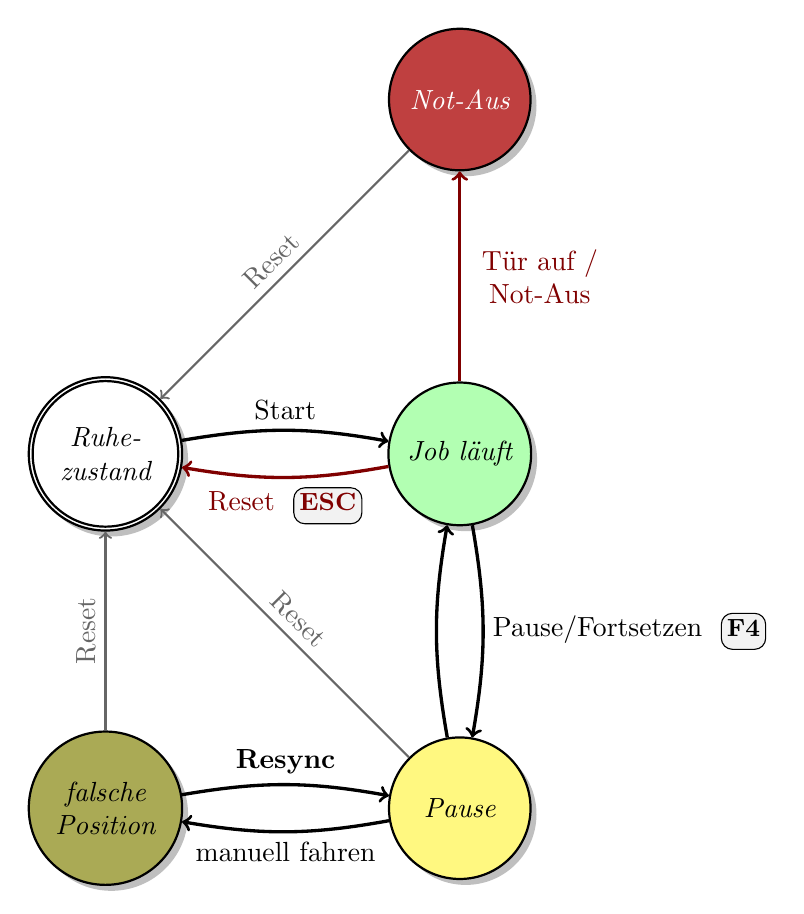
\begin{tikzpicture}[node distance=4.5cm,auto]
\colorlet{dunkelrot}{red!50!black}
\tikzstyle{zustand}=[shape=circle,draw,text width=1.5cm,text centered,thick,drop shadow,font=\itshape]; 
\tikzstyle{pf}=[->,very thick,every node/.style={anchor=south,text centered}]
\tikzstyle{pfHinRueck}=[pf,<->]

\node[zustand,fill=white] (ruhe) {Ruhe\-zustand};
\node[circle,text width=1.6cm,draw,thick] at (ruhe) {}; % innere zweite Umrandung - sieht so hübscher aus als mit der Option "double"
%\node[right of=ruhe] (platzhalter1) {}; % Lücke zwischen Ruhezustand und Job läuft
\node[zustand,right of=ruhe,fill=green!30!white] (aktiv) {Job läuft};

\node[zustand,above of=aktiv,fill=red!50!gray,text=white] (notaus) {Not-Aus};

\node[zustand,below of=aktiv,fill=yellow!50!white] (pause) {Pause};
\colorlet{schmutziggelb}{rgb:yellow,1;white,1;black,1}

\node[zustand,left of=pause,fill=schmutziggelb] (pauseVerschoben) {falsche Position};

\draw[pf,bend left=10] (ruhe) to node {Start}  (aktiv);
\draw[pf,bend left=10,dunkelrot] (aktiv) to node[anchor=north] {Reset \knopf{ESC}} (ruhe);

\draw[pf,bend left=10] (aktiv) to node[right] {Pause/Fortsetzen \knopf{F4}} (pause);
\draw[pf,bend left=10] (pause) to  (aktiv);
\draw[pf,bend left=10] (pause) to node[anchor=north] {manuell fahren} (pauseVerschoben) ;
\draw[pf,bend left=10] (pauseVerschoben) to node {\textbf{Resync}} (pause);

\draw[pf,dunkelrot] (aktiv) to node[right,text width=5em] {Tür auf /\\Not-Aus} (notaus);

\tikzstyle{unwichtig}=[color=black!60!white,thick]
\draw[pf,unwichtig] (notaus) to  node[sloped] {Reset} (ruhe);

\draw[pf,unwichtig,sloped] (pause) to node[sloped] {Reset} (ruhe);
\draw[pf,unwichtig,sloped] (pauseVerschoben) to node {Reset} (ruhe);
\end{tikzpicture}
\end{center}

Damit nach einer Unterbrechung wieder vom gleichen Zustand aus fortgesetzt wird, auch wenn man den Fräser zwischendurch manuell verfahren hat, erscheint nach \knopf{Start} der Resync-Dialog.

Jeder der Knöpfe steht für eine Variable. Grün heißt, dass der Zustand passend zum Fortsetzen ist. Draufklicken schaltet den Zustand um bzw. fährt zum passenden Fortsetzungspunkt.

\textbf{Bei Verwirrung geht stattdessen auch:} \knopf{Reset} setzt das Programm auf den Anfang zurück, jetzt kann man es nochmal vom Start aus laufen lassen. Es fräst dann anfangs in der Luft, das stört aber nicht weiter.

Die sinnvolle Reihenfolge beim Bedienen ist:
\begin{enumerate}
 \item Nach \knopf{Start} ist der Resync-Dialog links erschienen.
		\item Geschwindigkeit F (Textfeld), mit der zur Z-Höhe zurückgefahren wird, sollte auf 100 stehen (Kriechgang), sonst Crashgefahr.\\ Diese Geschwindigkeit gilt nicht für X/Y!
		\item Spindel an: \knopf{S}
		\item Kühlung an: \knopf{M8} kann manchmal auch rot sein, Hauptsache sie ist an
		\item Die Position kann auch wie gewohnt per Tastatur verfahren werden.
		\item Wenn die X/Y-Position nicht stimmt (Knopf mit roter Schrift), am besten erstmal den Fräser mit BildHoch aus dem Werkstück rausfahren, damit man nicht aus Versehen quer durchs Werkstück fährt.
			(Vorsicht bei sehr speziellen Fräserformen wie Gewindefräser, Kugelfräser o.\,ä.: Dabei kann es sein, dass man nicht einfach geradeaus hochfahren darf.)
		\item Position anfahren: \knopf{X}, \knopf{Y} (Abbrechen mit Esc)
		\item Danach Position \knopf{Z} anfahren (Abbrechen mit Esc)
		\item Erst wenn alles auf grün: \knopf{Start}
\end{enumerate}

\subsection{Auftragsende, Bezahlung}
\begin{enumerate}
 \item Die abgelaufene Zeit wird angezeigt. Eine grobe Vorhersage wird auch nach dem nach dem Neuladen der Datei angezeigt.
 \item Eingeben und Bezahlen im Kassenterminal: Grundpreis + Minuten Fräse + Minuten Fräser (wenn Fräser vom Lab genutzt wurde)  bzw. Stückpreis Fräser (wenn Fräser vom Lab genutzt wurde und kaputt ging)
 \item Aufräumen wie unter \ref{ordnung} beschrieben.
\end{enumerate}


\section{Fehlerbehebung}

\subsection{Werkzeugwechsel während Job wird nicht unterstützt}
Wenn ein Fehler \enquote{Werkzeugwechsel während Job wird nicht unterstützt.} kommt, dann passt die aktuell geladene Werkzeugnummer nicht zur vom Programm erwarteten Werkzeugnummer. Abhilfe: Reset und den kompletten Einrichtvorgang (Werkzeug wechseln, Länge, Z-Null) mit der korrekten Werkzeugnummer wiederholen.

\subsection{Notaus löst aus}
Eine Schutzabschaltung kann u.\,a. folgende Gründe haben:
\begin{itemize}
	\item Umrichterfehler
	\item Kühlaggregat aus / Fehler
	\item HSK-Einsatz nicht korrekt eingelegt (Lampe \enquote{Werkzeug OK}?)
	\item Notaus-Knopf gedrückt
	\item Fehlbedienung
\end{itemize}

\subsection{Maschine dreht nur bis ca. 15000 Umdrehungen hoch und schaltet dann ab}
Der Umrichter hat zwei Profile, die in unterschiedlichen Drehzahlbereichen ideal funktionieren.
\begin{itemize}
	\item Profil 1: 0 bis 18000 rpm, im unteren Bereich nicht volles Drehmoment möglich. 
	\item Profil 2: 0 bis ca. 15000 rpm, darüber steigt der Umrichter aus. Volles Drehmoment bis 12000 rpm
\end{itemize}
In über 90\% aller Fälle reicht Profil 1 aus, auch z.B. für 10mm Fräser ZOX Vollnut in Aluminium (getestet). Für den Fall, dass das drehmomenterhöhte Profil im Umrichter geladen und dann verwendet wurde, ist es \textbf{AUF JEDEN FALL} nach der Arbeit wieder auf Profil 1 zurück zu stellen. Vor der Arbeit ist zu kontrollieren, dass im Umrichterdisplay oben rechts \enquote{1(1)} steht, da dies auf Profil 1 hinweist.

Hintergrund:\\
Der Umrichter will den Motor nur bis leicht über den Anfang der Feldschwächung betreiben, der bei unserer Spindel bei 12000 rpm beginnt. Daher wird dem Umrichter im Profil 1 für höhere Drehzahlen vorgegaukelt, dass die Feldschwächung erst bei 24000 rpm anfängt. Damit steuert der Umrichter die den Motor auf zu geringer Spannung aber korrekter Frequenz. So ist zwar das Drehmoment, welches eine Funktion des Stromes ist, nicht maximal möglich, aber die Drehzahl sehr wohl. Theoretisch wären so 24000 rpm möglich, die Drehzahl wurde aber wegen Schwierigkeiten mit der Umrichter-Regelung auf 18.000 rpm begrenzt.

\subsection{Schrittverlust}
Bei zu großer Kraft kann die Fräse Schritte verlieren, d.h. es gibt jetzt einen Versatz zwischen der echten Position und der, die die Steuerung haben will. Das kann die Steuerung nicht merken! Abhilfe ist im Zweifelsfall eine erneute Referenzfahrt, das kann nie schaden und zeigt an, ob es Schrittverlust gab. Wenn nur 1 Schritt Verlust angezeigt wird, kann man das als Messfehler ignorieren.

\subsection{Fräserbruch}
\begin{itemize}
 \item Schrittverlust ist zu befürchten $\rightarrow$ Referenzfahrt!
 \item Vorderes abgebrochenes Teil des Fräsers anschauen: optisch in Ordnung? verklebt (Alu/Kunststoff)? noch scharf?
 \item Restliche Hartmetallteile aus dem Werkstück entfernen, sonst wird der nächste Fräser bei Berührung gleich wieder zerstört.
 \item Aufbauschneide? wenn ja: mehr KSS oder richtigen Fräser verwenden!
 \item Aufspannung starr genug? Blech wird gerne hochgezogen, sodass die Zustellung zu groß wird oder den Fräser einklemmt.
 \item Ausreichend Schmierung?
 \item Zustellung verringern bei gleichem Vorschub, oder Vorschub verringern. Hat beides seine Vor- und Nachteile.
 \item Stege zu klein $\rightarrow$ Werkstück verschiebt sich und klemmt in den Fräser $\rightarrow$ Stege größer machen oder umspannen
 \item Falsche Schnittgeschwindigkeit? Im Datenblatt des Fräsers nachschauen und nachrechnen.
 \end{itemize}


\subsection{MCA/TCA Collision}
Werkzeug vermessen? Nullpunkt korrekt?

Die angezeigte Koordinate ist nicht immer die Ursache der Fehlermeldung.

MCA: Fräsung zu tief ($<2$\,mm vom Tisch) oder außerhalb des Verfahrbereichs der Maschine. Beachte: Ein Fräser, der kürzer als 30\,mm herausragt, kommt nicht bis an den Tisch runter, weil die Z-Achse zu kurz ist!

TCA: Kollision mit \enquote{verbotenem Bereich} rund um den Längenmesstaster, also zu nahe dran. Mehr Abstand halten.

\section{Grundlagen}
\todo{ein kurzer Abschnitt über die nötigen Daten, und Begriffe erklären. Planfräsen, Nutfräsen, Stege,...}

\subsection{Schnittdaten ermitteln}

Die Lebensdauer des Fräsers und Qualität des Ergebnisses hängt stark davon ab, dass Drehzahl und Vorschub passend gewählt werden.

\paragraph{Übliche Werkstoffe} Gute Startwerte für Kunststoff bis Metall liefert das von der Firma Hoffmann vertriebene Zerspanungshandbuch, welches auch online erhältlich ist. Ein Standardfräser ist dort unter Schaftfräser VHM (bzw. HSS) unbeschichtet zu finden, normales Fräsen als Nutfräsen mit Eingriffsbreite $a_e=1\cdot D$, und Eingriffstiefe $a_p=1 \cdot D$. Für kleinere Fräser (3mm und kleiner) sollte man mit der Eingriffstiefe eher auf $D/2$ runtergehen.

\begin{enumerate}
	\item Nachschauen: Fräserdurchmesser $D$, Schneidenzahl $z$ (1 ... 5).
	\item Schnittgeschwindigkeit $v_c$ (in m/min) aus der fräserspezifischen Tabelle für das gewünschte Material ablesen.
	\item Gewünschte Drehzahl $n$ in Umdrehungen pro Minute (1/min, auch rpm genannt) ausrechnen.\\
		Es gilt $n=\frac{v_c}{\pi D}$ bzw. $v_c=\pi n D$.
	\item Echte Drehzahl $n$ bestimmen: Wenn möglich, dann die gewünschte Drehzahl, ansonsten so hoch wie möglich. Maximal möglich sind 18.000 rpm, außerdem muss der Fräser dafür zugelassen sein.
	\item Vorschubgeschwindigkeit $v_f$ in mm/min bestimmen: In der Tabelle ist meist der spezifische Vorschub $f_z=\frac{v_f}{z\cdot n}$ pro Schneide und Umdrehung angegeben. Ausnahme sind Bohrer, dort ist meist der Vorschub pro Umdrehung $f=\frac{v_f}{n}$ angegeben. \\
		Formel: $v_f = n z f_z$ bzw. $v_f=n f$.
	\item Übliche Werte für den Vorschub sind 350 (langsam) bis 3000 mm/min (echt schnell). Mehr als 3000 mm/min kann die Maschine nicht.
	\item Die Tabellenwerte gelten für ideale Aufspannung, z.B. ein mit Schraubstock oder Spannpratzen festgezogenes Stück 10mm dickes Aluminium. Auch sollte der Fräserschaft nicht unnötig weit aus dem Spannfutter herausragen. Bei schlechter Aufspannung bzw. dünnem Material kann die Eintauchtiefe auf $D/2$ reduziert werden. Auch kann der Vorschub halbiert werden, wobei das nicht unbedingt besser für den Fräser ist. Bei viel zu geringem Vorschub reibt der Fräser nur noch, weil kein sauberer Span zustandekommt.

		Die Qualität einer Aufspannung prüft man am Besten am Klang durch Daraufklopfen mit dem Finger oder Schraubenschlüssel. Je weicher die Aufspannung ist, umso deutlicher merkt man einen Unterschied zwischen dem festgespannten Rand und der Mitte des Materials. Bei guter Aufspannung sollte sich außerdem nichts bewegen, wenn man etwas drückt oder zieht. Bei dünnem Blech kann die Aufspannung nicht beliebig gut sein, weil man ab einer gewissen Andruckkraft das Blech verbiegt und zerquetscht.
		
		Einen groben Anhaltspunkt für den Vorschub liefert das Aussehen der Späne. Sie sollten beim Fräsen weder haarfein sein (zuviel Vorschub) noch grobe Brocken oder gar lange Bänder (zuwenig Vorschub).
\end{enumerate}

Die so gewonnenen Werte speichern wir unter Nutfräsen ab. Dazu sollte immer eine Beschreibung kommen, ob und wann und an was genau sie getestet wurden. Diese Werte werden auch für das Taschenfräsen verwendet, wobei man als seitliche Zustellung zwischen den Fräserbahnen 40\% der Fräserbreite angeben sollte.

\paragraph{Holz} Für Holz benötigt man extrem hohe Schnittgeschwindigkeiten und daher eine hohe Drehzahl: Solange der Fräser dafür zugelassen ist (Aufdruck oder Datenblatt), 18.000 rpm bis etwa 8 mm Durchmesser. Vorschub mit 1000 mm/min anfangen (ab etwa 4mm Durchmesser) und solange erhöhen, bis das Holz zerfetzt wird oder andere Probleme auftreten. Wenn die Ränder der Fräsbahn verkohlen, ist der Vorschub zu gering, oder der Fräser stumpf geworden.


\ccLicense{fraese-einweisung}{Einweisung Fräse}

\end{document}
